\documentclass[10pt,a4paper,onecolumn]{article}
\usepackage{marginnote}
\usepackage{graphicx}
\usepackage{xcolor}
\usepackage{authblk,etoolbox}
\usepackage{titlesec}
\usepackage{calc}
\usepackage{tikz}
\usepackage{hyperref}
\hypersetup{colorlinks,breaklinks,
            urlcolor=[rgb]{0.0, 0.5, 1.0},
            linkcolor=[rgb]{0.0, 0.5, 1.0}}
\usepackage{caption}
\usepackage{tcolorbox}
\usepackage{amssymb,amsmath}
\usepackage{ifxetex,ifluatex}
\usepackage{seqsplit}
\usepackage{fixltx2e} % provides \textsubscript
\usepackage[
  backend=biber,
%  style=alphabetic,
%  citestyle=numeric
]{biblatex}
\bibliography{paper.bib}



% --- Page layout -------------------------------------------------------------
\usepackage[top=3.5cm, bottom=3cm, right=1.5cm, left=1.0cm,
            headheight=2.2cm, reversemp, includemp, marginparwidth=4.5cm]{geometry}

% --- Default font ------------------------------------------------------------
% \renewcommand\familydefault{\sfdefault}

% --- Style -------------------------------------------------------------------
\renewcommand{\bibfont}{\small \sffamily}
\renewcommand{\captionfont}{\small\sffamily}
\renewcommand{\captionlabelfont}{\bfseries}

% --- Section/SubSection/SubSubSection ----------------------------------------
\titleformat{\section}
  {\normalfont\sffamily\Large\bfseries}
  {}{0pt}{}
\titleformat{\subsection}
  {\normalfont\sffamily\large\bfseries}
  {}{0pt}{}
\titleformat{\subsubsection}
  {\normalfont\sffamily\bfseries}
  {}{0pt}{}
\titleformat*{\paragraph}
  {\sffamily\normalsize}


% --- Header / Footer ---------------------------------------------------------
\usepackage{fancyhdr}
\pagestyle{fancy}
\fancyhf{}
%\renewcommand{\headrulewidth}{0.50pt}
\renewcommand{\headrulewidth}{0pt}
\fancyhead[L]{\hspace{-0.75cm}\includegraphics[width=5.5cm]{C:/Users/npjun/AppData/Local/R/win-library/4.3/rticles/rmarkdown/templates/joss/resources/JOSS-logo.png}}
\fancyhead[C]{}
\fancyhead[R]{}
\renewcommand{\footrulewidth}{0.25pt}

\fancyfoot[L]{\footnotesize{\sffamily Piñeiro-Juncal et.
al., (2025). BlueCarbon R package: Estimation of Organic Carbon Stocks
and Sequestration Rates From Soil Core
Data. \textit{Journal of Open Source Software}, (), . \href{https://doi.org/}{https://doi.org/}}}


\fancyfoot[R]{\sffamily \thepage}
\makeatletter
\let\ps@plain\ps@fancy
\fancyheadoffset[L]{4.5cm}
\fancyfootoffset[L]{4.5cm}

% --- Macros ---------

\definecolor{linky}{rgb}{0.0, 0.5, 1.0}

\newtcolorbox{repobox}
   {colback=red, colframe=red!75!black,
     boxrule=0.5pt, arc=2pt, left=6pt, right=6pt, top=3pt, bottom=3pt}

\newcommand{\ExternalLink}{%
   \tikz[x=1.2ex, y=1.2ex, baseline=-0.05ex]{%
       \begin{scope}[x=1ex, y=1ex]
           \clip (-0.1,-0.1)
               --++ (-0, 1.2)
               --++ (0.6, 0)
               --++ (0, -0.6)
               --++ (0.6, 0)
               --++ (0, -1);
           \path[draw,
               line width = 0.5,
               rounded corners=0.5]
               (0,0) rectangle (1,1);
       \end{scope}
       \path[draw, line width = 0.5] (0.5, 0.5)
           -- (1, 1);
       \path[draw, line width = 0.5] (0.6, 1)
           -- (1, 1) -- (1, 0.6);
       }
   }

% --- Title / Authors ---------------------------------------------------------
% patch \maketitle so that it doesn't center
\patchcmd{\@maketitle}{center}{flushleft}{}{}
\patchcmd{\@maketitle}{center}{flushleft}{}{}
% patch \maketitle so that the font size for the title is normal
\patchcmd{\@maketitle}{\LARGE}{\LARGE\sffamily}{}{}
% patch the patch by authblk so that the author block is flush left
\def\maketitle{{%
  \renewenvironment{tabular}[2][]
    {\begin{flushleft}}
    {\end{flushleft}}
  \AB@maketitle}}
\makeatletter
\renewcommand\AB@affilsepx{ \protect\Affilfont}
%\renewcommand\AB@affilnote[1]{{\bfseries #1}\hspace{2pt}}
\renewcommand\AB@affilnote[1]{{\bfseries #1}\hspace{3pt}}
\makeatother
\renewcommand\Authfont{\sffamily\bfseries}
\renewcommand\Affilfont{\sffamily\small\mdseries}
\setlength{\affilsep}{1em}


\ifnum 0\ifxetex 1\fi\ifluatex 1\fi=0 % if pdftex
  \usepackage[T1]{fontenc}
  \usepackage[utf8]{inputenc}

\else % if luatex or xelatex
  \ifxetex
    \usepackage{mathspec}
  \else
    \usepackage{fontspec}
  \fi
  \defaultfontfeatures{Ligatures=TeX,Scale=MatchLowercase}

\fi
% use upquote if available, for straight quotes in verbatim environments
\IfFileExists{upquote.sty}{\usepackage{upquote}}{}
% use microtype if available
\IfFileExists{microtype.sty}{%
\usepackage{microtype}
\UseMicrotypeSet[protrusion]{basicmath} % disable protrusion for tt fonts
}{}

\usepackage{hyperref}
\hypersetup{unicode=true,
            pdftitle={BlueCarbon R package: Estimation of Organic Carbon Stocks and Sequestration Rates From Soil Core Data},
            pdfborder={0 0 0},
            breaklinks=true}
\urlstyle{same}  % don't use monospace font for urls
\usepackage{graphicx,grffile}
\makeatletter
\def\maxwidth{\ifdim\Gin@nat@width>\linewidth\linewidth\else\Gin@nat@width\fi}
\def\maxheight{\ifdim\Gin@nat@height>\textheight\textheight\else\Gin@nat@height\fi}
\makeatother
% Scale images if necessary, so that they will not overflow the page
% margins by default, and it is still possible to overwrite the defaults
% using explicit options in \includegraphics[width, height, ...]{}
\setkeys{Gin}{width=\maxwidth,height=\maxheight,keepaspectratio}
\IfFileExists{parskip.sty}{%
\usepackage{parskip}
}{% else
\setlength{\parindent}{0pt}
\setlength{\parskip}{6pt plus 2pt minus 1pt}
}
\setlength{\emergencystretch}{3em}  % prevent overfull lines
\setcounter{secnumdepth}{0}
% Redefines (sub)paragraphs to behave more like sections
\ifx\paragraph\undefined\else
\let\oldparagraph\paragraph
\renewcommand{\paragraph}[1]{\oldparagraph{#1}\mbox{}}
\fi
\ifx\subparagraph\undefined\else
\let\oldsubparagraph\subparagraph
\renewcommand{\subparagraph}[1]{\oldsubparagraph{#1}\mbox{}}
\fi


% tightlist command for lists without linebreak
\providecommand{\tightlist}{%
  \setlength{\itemsep}{0pt}\setlength{\parskip}{0pt}}


% Pandoc citation processing
\newlength{\cslhangindent}
\setlength{\cslhangindent}{1.5em}
\newlength{\csllabelwidth}
\setlength{\csllabelwidth}{3em}
\newlength{\cslentryspacingunit} % times entry-spacing
\setlength{\cslentryspacingunit}{\parskip}
% for Pandoc 2.8 to 2.10.1
\newenvironment{cslreferences}%
  {}%
  {\par}
% For Pandoc 2.11+
\newenvironment{CSLReferences}[2] % #1 hanging-ident, #2 entry spacing
 {% don't indent paragraphs
  \setlength{\parindent}{0pt}
  % turn on hanging indent if param 1 is 1
  \ifodd #1
  \let\oldpar\par
  \def\par{\hangindent=\cslhangindent\oldpar}
  \fi
  % set entry spacing
  \setlength{\parskip}{#2\cslentryspacingunit}
 }%
 {}
\usepackage{calc}
\newcommand{\CSLBlock}[1]{#1\hfill\break}
\newcommand{\CSLLeftMargin}[1]{\parbox[t]{\csllabelwidth}{#1}}
\newcommand{\CSLRightInline}[1]{\parbox[t]{\linewidth - \csllabelwidth}{#1}\break}
\newcommand{\CSLIndent}[1]{\hspace{\cslhangindent}#1}



\title{BlueCarbon R package: Estimation of Organic Carbon Stocks and
Sequestration Rates From Soil Core Data}

        \author[1]{Nerea Piñeiro-Juncal}
          \author[2]{Julen Astigarraga}
          \author[3]{Valentina Costa}
          \author[4]{Márcio Martins}
          \author[5]{Francisco Rodríguez-Sánchez}
    
      \affil[1]{Centro de Investigacions Mariñas da Universidade de
Vigo. Departamento de Xeocencias Mariñas e Ordenación do Territorio,
Facultade de Ciencias do Mar, Campus Lagoas Marcosende, Universidad de
Vigo, Vigo, Spain}
      \affil[2]{Universidad de Alcalá, Grupo de Ecología Forestal y
Restauración (FORECO), Departamento de Ciencias de la Vida, Spain}
      \affil[3]{Affil3}
      \affil[4]{Affil4}
      \affil[5]{Departamento de Biología Vegetal y Ecología, Universidad
de Sevilla, Spain}
  \date{\vspace{-5ex}}

\begin{document}
\maketitle

\marginpar{
  %\hrule
  \sffamily\small

  {\bfseries DOI:} \href{https://doi.org/}{\color{linky}{}}

  \vspace{2mm}

  {\bfseries Software}
  \begin{itemize}
    \setlength\itemsep{0em}
    \item \href{}{\color{linky}{Review}} \ExternalLink
    \item \href{}{\color{linky}{Repository}} \ExternalLink
    \item \href{}{\color{linky}{Archive}} \ExternalLink
  \end{itemize}

  \vspace{2mm}

  {\bfseries Submitted:} \\
  {\bfseries Published:} 

  \vspace{2mm}
  {\bfseries License}\\
  Authors of papers retain copyright and release the work under a Creative Commons Attribution 4.0 International License (\href{http://creativecommons.org/licenses/by/4.0/}{\color{linky}{CC-BY}}).
}

Correspondence:

Nerea Piñeiro-Juncal, University of Vigo, Vigo, Spain. Email:
\href{mailto:np.juncal@gmail.com}{\nolinkurl{np.juncal@gmail.com}}

\hypertarget{summary}{%
\section{Summary}\label{summary}}

\emph{\texttt{BlueCarbon}} facilitate the estimation of organic carbon
stocks and sequestration rates from soil/sediment cores from blue carbon
ecosystems. It contains seven main functions to estimate the compaction
of cores, mathematically correct core compaction, estimate sample
thickness, estimate organic carbon content from organic matter content,
estimate organic carbon stocks and sequestration rates and visualize the
error of stock extrapolation.

\hypertarget{statement-of-need}{%
\section{Statement of Need}\label{statement-of-need}}

Coastal blue carbon ecosystems have earn a large attention for their
role as sinks of organic carbon. In the last decade, publications about
blue carbon research have grown exponentially, including many studies
reporting soil organic carbon stocks and sequestration rates ().
Although there are many soil sampling strategies, estimation
methodologies are fairly homogeneous, following the protocol published
by the Blue Carbon initiative (). However, and although many blue carbon
researchers work in R and it is becoming more comon to publish the code
used, there is no R library with functions especifically for blue carbon
estimations. This library aims to standardize and automate the main
estimations to get soil/sediment blue carbon stocks and sequestration
rates from raw field and laboratory data.

\hypertarget{design}{%
\section{Design}\label{design}}

The BLueCarbon library contains seven main functions to deal with core
compaction (estimate the compaction of cores and mathematically correct
core compaction), transform laboratory data (estimate sample thickness
and estimate organic carbon content from organic matter content) and
estimate organic carbon stocks and sequestration rates (estimate organic
carbon stocks and sequestration rates and visualize the error of stock
extrapolation).

\begin{enumerate}
\def\labelenumi{\arabic{enumi}.}
\item
  estimate\_compaction
\item
  decompact
\item
  estimate\_oc
\item
  estimate\_h
\item
  estimate\_oc\_stocks
\item
  test\_extrapolation
\item
  estimate\_seq\_rate
\end{enumerate}

\begin{figure}
\centering
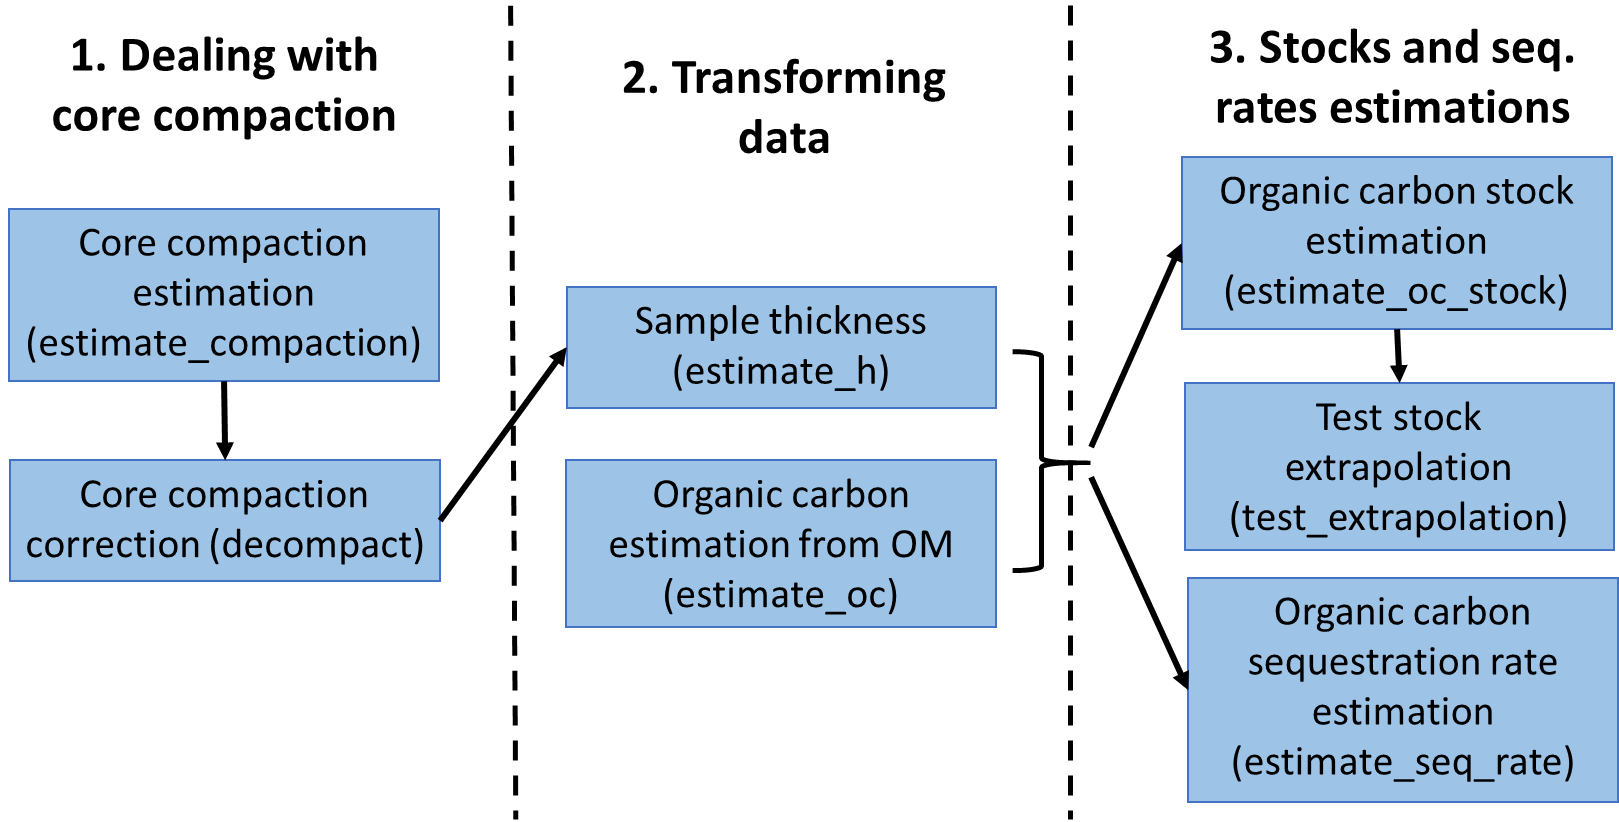
\includegraphics{images/BC_workflow-01.png}
\caption{Blue Carbon library workflow}
\end{figure}

\hypertarget{estimate_compaction---estimate-core-compaction}{%
\paragraph{\texorpdfstring{\textbf{\emph{estimate\_compaction}}
\textbf{- Estimate Core
Compaction}}{estimate\_compaction - Estimate Core Compaction}}\label{estimate_compaction---estimate-core-compaction}}

Sampling soil cores by manual percussion usually leads to the compaction
of the material retrieved. This function will estimate the percentage of
compaction from measurements taken in the field after inserting the
corer tube and before extracting it: length of the corer tube
(sampler\_length), distance between the surface of the soil and the top
of the tube in the outside (external\_distance) and distance between the
surface of the soil and the top of the tube in the inside of the tube
(internal\_distance).

\begin{figure}
\centering
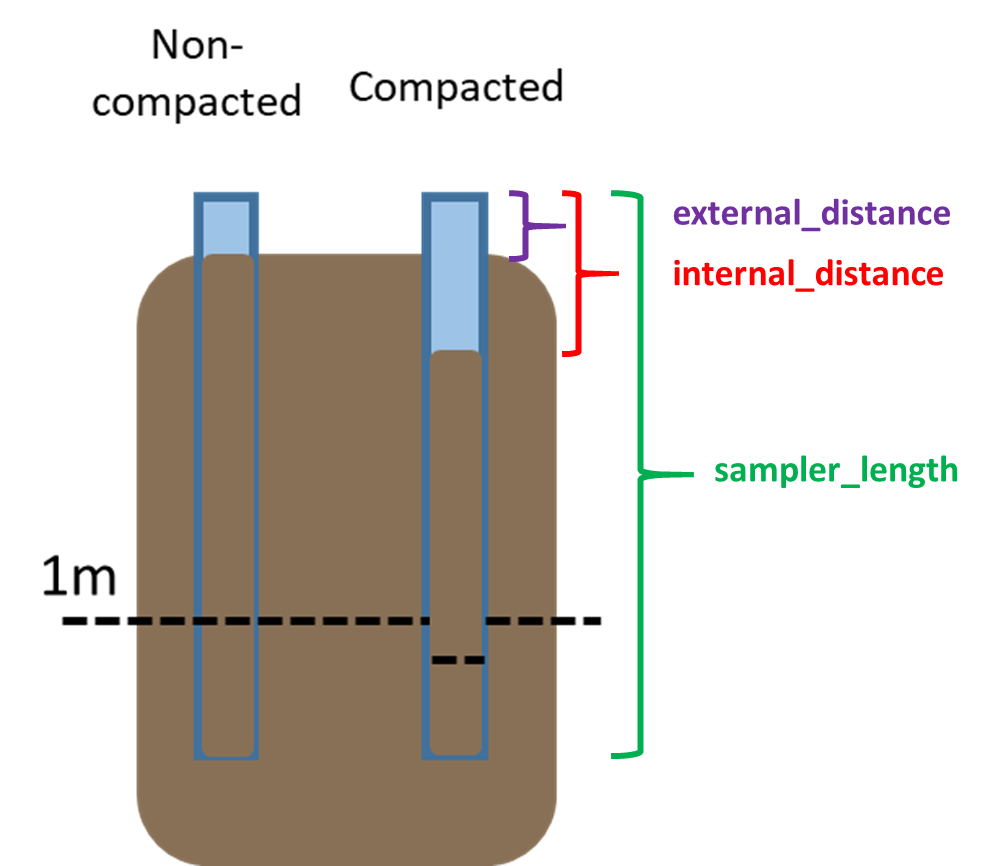
\includegraphics[width=4.16667in,height=\textheight]{images/compaction-01.png}
\caption{Soil compaction from field sampling}
\end{figure}

\hypertarget{decompact---calculate-sediment-properties-after-decompaction}{%
\paragraph{\texorpdfstring{\textbf{\emph{decompact}} \textbf{- Calculate
sediment properties after
decompaction}}{decompact - Calculate sediment properties after decompaction}}\label{decompact---calculate-sediment-properties-after-decompaction}}

Core compaction derived from field extraction can be mathematically
correct to estimate the original depth of the samples. This function
will apply a linear correction (all the core material is assumed to have
been compacted equally) to correct sample depth and, if provided, dry
bulk density.

\hypertarget{estimate_oc---organic-carbon-content-estimation-from-organic-carbon-data}{%
\paragraph{\texorpdfstring{\textbf{\emph{estimate\_oc}} \textbf{-
Organic carbon content estimation from organic carbon
data}}{estimate\_oc - Organic carbon content estimation from organic carbon data}}\label{estimate_oc---organic-carbon-content-estimation-from-organic-carbon-data}}

There is linear correlation between organic carbon and organic matter
content. This correlation can change between ecosystems and sampling
sites due to changes in organic matter composition among other factors.
This function model a linear correlation between organic matter and
organic carbon content in your samples and predict the content of
organic carbon for those samples were there is no organic carbon values.
Estimation of organic carbon is done by means of linear regressions on
log(organic carbon) \textasciitilde{} log(organic matter). It gives back
a organic carbon value for each organic matter value provided. If there
is a organic carbon value for that sample it return the same value,
else, generates a model for that site, else, model for specie, else,
model for that ecosystem. If a model can not be created due to the low
number of samples (\textless10) it uses the equations in
\texttt{Fourqurean:2012} for seagrasses, Maxwell et al. (2023) for salt
marshes and Piñeiro-Juncal in prepp for mangroves to estimate the
organic carbon. It is unlikely, but possible, that a model will predict
a higher organic carbon than organic matter content. This is not
possible in nature. If this is the case the function will give a warning
and it is recommended to discard that model.

\hypertarget{estimate_h---sample-thickness-estimation}{%
\paragraph{\texorpdfstring{\textbf{\emph{estimate\_h}} \textbf{- Sample
thickness
estimation}}{estimate\_h - Sample thickness estimation}}\label{estimate_h---sample-thickness-estimation}}

For those cores were only selected samples were measured it is necessary
to assign a carbon density to the empty spaces before the estimation the
total stock. This function checks for gaps between samples and, if any,
divide this space between the previous and next sample to return sample
thickness without gaps in the core. The middle point between one sample
and the other is estimated from the bottom of the previous sample to the
top of the next sample, and not form the middle point of one sample to
the middle part of the next, as this would inequality distribute the
gaps between samples if the samples have different thickness. The stock
and sequestration rate estimation functions (estimate\_oc\_stock and
estimate\_seq\_rate) have this function incorporated and it is not
necessary to run it beforehand.

\begin{figure}
\centering
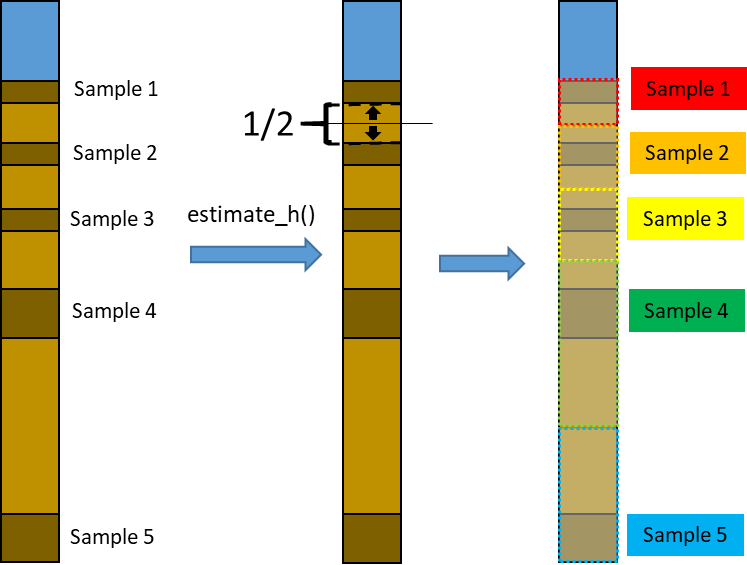
\includegraphics[width=4.97917in,height=\textheight]{images/estimate_h().png}
\caption{Gap distribution between samples to estimate accumulated
organic carbon mass.}
\end{figure}

\hypertarget{estimate_oc_stock---organic-carbon-stock-estimation}{%
\paragraph{\texorpdfstring{\textbf{\emph{estimate\_oc\_stock}} \textbf{-
Organic carbon stock
estimation}}{estimate\_oc\_stock - Organic carbon stock estimation}}\label{estimate_oc_stock---organic-carbon-stock-estimation}}

Estimates carbon stocks from soil core data down to a specified depth,
100 cm by default. If the core does not reach the desired depth, it
extrapolates the stock from a linear model between accumulated mass of
organic carbon and depth.

\begin{figure}
\centering
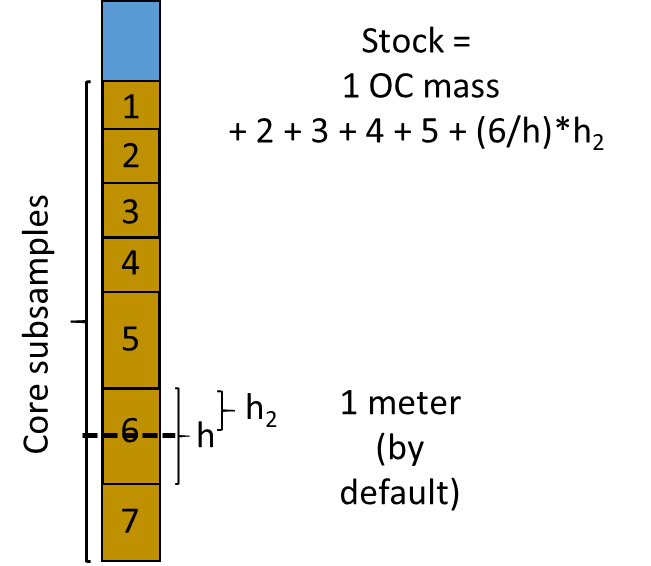
\includegraphics[width=3.83333in,height=\textheight]{images/estimate_stock.png}
\caption{OC stock estimation diagram}
\end{figure}

\hypertarget{test_extrapolation---visualize-the-error-of-stock-extrapolation}{%
\paragraph{\texorpdfstring{\textbf{\emph{test\_extrapolation}} \textbf{-
Visualize the error of stock
extrapolation}}{test\_extrapolation - Visualize the error of stock extrapolation}}\label{test_extrapolation---visualize-the-error-of-stock-extrapolation}}

This function subset those cores that reach the desired depth, estimates
the stock (observed stock), estimate the stock from the linear relation
of organic carbon accumulated mass and depth using the 90, 75, 50 and
25\% top length of the indicated desired depth. Compares the observed
stock with the estimated stocks by extrapolation. This function requires
that some of you core do reach the desired depth.

\hypertarget{estimate_seq_rate---organic-carbon-sequestration-rates-estimation}{%
\paragraph{\texorpdfstring{\textbf{\emph{estimate\_seq\_rate}} \textbf{-
Organic carbon sequestration rates
estimation}}{estimate\_seq\_rate - Organic carbon sequestration rates estimation}}\label{estimate_seq_rate---organic-carbon-sequestration-rates-estimation}}

Estimate the average organic carbon sequestration rate to the soil in a
indicated time frame (by default last 100 years) from the organic carbon
concentration and the age of the samples.

\hypertarget{availability}{%
\section{Availability}\label{availability}}

The library is available xxxx.
\href{https://github.com/EcologyR/BlueCarbon/}{Browse the source core}
To install it\ldots{} The library and tutorials can be accessed
\href{https://ecologyr.github.io/BlueCarbon/}{here} and a workshop
recording and a step-by-step tutorial walkthrough are available
\href{https://www.youtube.com/watch?v=XCrrR3_MSHc\&ab_channel=EcoinformaticaAEET}{here}.

\hypertarget{acknowledgements}{%
\section{Acknowledgements}\label{acknowledgements}}

The development of this software has been funded by Fondo Europeo de
Desarrollo Regional (FEDER) and Consejería de Transformación Económica,
Industria, Conocimiento y Universidades of Junta de Andalucía (proyecto
US-1381388 led by Francisco Rodríguez Sánchez, Universidad de Sevilla).
NPJ was supported by a Juan de la Cierva fellowship (JDC2022-048342-I,
funded by MCIN/AEI/10.13039/501100011033 and the European Union
``NextGenerationEU''/PRTR''). JA acknowledges funding from the
CLIMB-FOREST Horizon Europe Project (No 101059888) that was funded by
the European Union.

\hypertarget{references}{%
\section{References}\label{references}}

Fourqureanet al.~(2012) Seagrass ecosystems as a globally significant
carbon stock. Nat. Geosci.5, 505--509.
\url{https://doi.org/10.1038/ngeo1477}

Maxwell et al.~(2023) Global dataset of soil organic carbon in tidal
marshes.Sci.Data 10,
1--14.\url{https://doi.org/10.1038/s41597-023-02633-x}

Piñeiro-Juncal et al.~(in prepp) Soil organic carbon preservation and
decay trends in tidal marsh, mangrove and seagrass blue carbon
ecosystems.

\hypertarget{refs}{}
\begin{CSLReferences}{1}{0}
\leavevmode\vadjust pre{\hypertarget{ref-Maxwell_2023}{}}%
Maxwell, T. L., Rovai, A. S., Adame, M. F., Adams, J. B., Álvarez-Rogel,
J., Austin, W. E. N., Beasy, K., et al. (2023). Global dataset of soil
organic carbon in tidal marshes. \emph{Scientific Data}, \emph{10}(1),
1--14.
doi:\href{https://doi.org/10.1038/s41597-023-02633-x}{10.1038/s41597-023-02633-x}

\end{CSLReferences}

\end{document}
